\label{3D-Druck}

Wir haben uns für den 3D-Druck entschieden, da uns einerseits der freie Zugang zu einer mechanischen Werkstatt gefehlt hat, andererseits der 3D-Druck uns die Möglichkeit gibt, ein absolut individuelles Gehäuse nach unseren Vorstellungen zu fertigen. Aus der Quelldatei vom \ac{CAD}-Programm wird mithilfe des Drucker-Eigenen Programms eine STL-Datei erstellt, in welcher die Sehnenhöhe und andere benötigten Daten, welche zum erfolgreichen Drucken des Gehäuses notwendig sind, definiert werden. Nach erfolgreicher Umwandlung wird der Druckprozess simuliert, um feststellen zu können, ob die Zeichnung so angefertigt kann, wie sie vorher gezeichnet wurde. In Abbildung \ref{fig:SimSTL} ist eine solche Simulation zu sehen, wie sie das Drucker-Eigene Programm ausgibt.

\begin{figure}[!hbt]
	\centering
	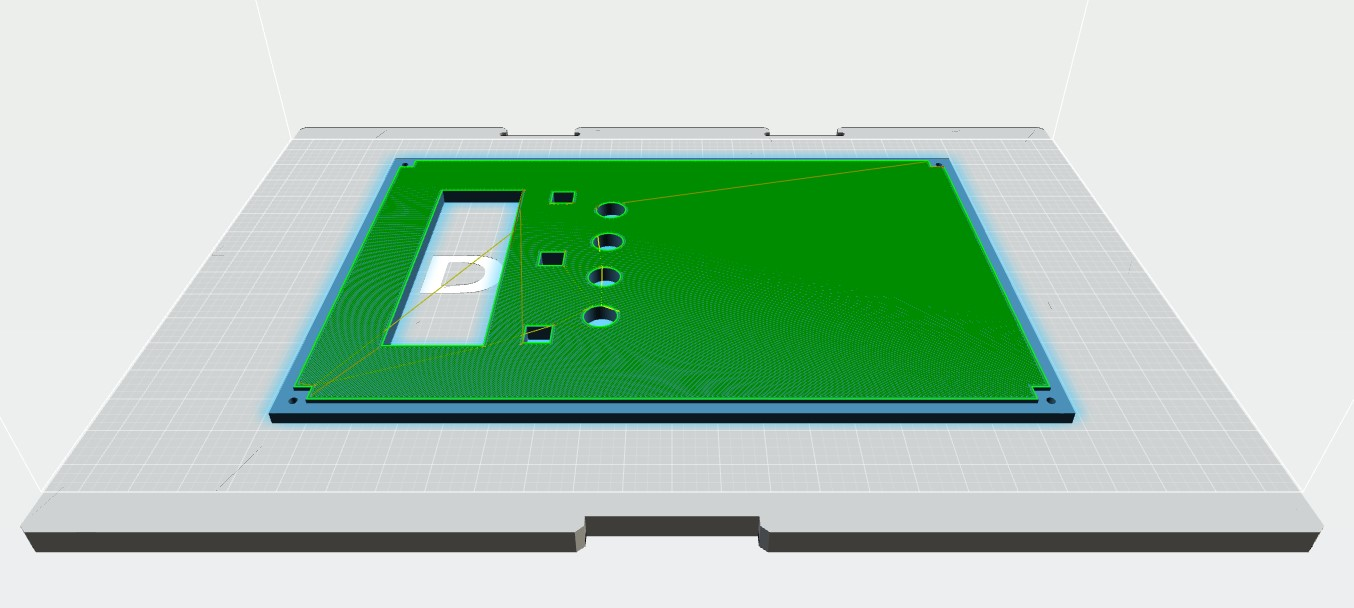
\includegraphics[width=0.9\linewidth]{Images/SimSTL}
	\footnotesize \\Quelle: eigene Aufnahme
	\caption{Simulation der \ac{STL}-Datei}
	\label{fig:SimSTL}
\end{figure}
